\documentclass[1p]{elsarticle_modified}
%\bibliographystyle{elsarticle-num}

%\usepackage[colorlinks]{hyperref}
%\usepackage{abbrmath_seonhwa} %\Abb, \Ascr, \Acal ,\Abf, \Afrak
\usepackage{amsfonts}
\usepackage{amssymb}
\usepackage{amsmath}
\usepackage{amsthm}
\usepackage{scalefnt}
\usepackage{amsbsy}
\usepackage{kotex}
\usepackage{caption}
\usepackage{subfig}
\usepackage{color}
\usepackage{graphicx}
\usepackage{xcolor} %% white, black, red, green, blue, cyan, magenta, yellow
\usepackage{float}
\usepackage{setspace}
\usepackage{hyperref}

\usepackage{tikz}
\usetikzlibrary{arrows}

\usepackage{multirow}
\usepackage{array} % fixed length table
\usepackage{hhline}

%%%%%%%%%%%%%%%%%%%%%
\makeatletter
\renewcommand*\env@matrix[1][\arraystretch]{%
	\edef\arraystretch{#1}%
	\hskip -\arraycolsep
	\let\@ifnextchar\new@ifnextchar
	\array{*\c@MaxMatrixCols c}}
\makeatother %https://tex.stackexchange.com/questions/14071/how-can-i-increase-the-line-spacing-in-a-matrix
%%%%%%%%%%%%%%%

\usepackage[normalem]{ulem}

\newcommand{\msout}[1]{\ifmmode\text{\sout{\ensuremath{#1}}}\else\sout{#1}\fi}
%SOURCE: \msout is \stkout macro in https://tex.stackexchange.com/questions/20609/strikeout-in-math-mode

\newcommand{\cancel}[1]{
	\ifmmode
	{\color{red}\msout{#1}}
	\else
	{\color{red}\sout{#1}}
	\fi
}

\newcommand{\add}[1]{
	{\color{blue}\uwave{#1}}
}

\newcommand{\replace}[2]{
	\ifmmode
	{\color{red}\msout{#1}}{\color{blue}\uwave{#2}}
	\else
	{\color{red}\sout{#1}}{\color{blue}\uwave{#2}}
	\fi
}

\newcommand{\Sol}{\mathcal{S}} %segment
\newcommand{\D}{D} %diagram
\newcommand{\A}{\mathcal{A}} %arc


%%%%%%%%%%%%%%%%%%%%%%%%%%%%%5 test

\def\sl{\operatorname{\textup{SL}}(2,\Cbb)}
\def\psl{\operatorname{\textup{PSL}}(2,\Cbb)}
\def\quan{\mkern 1mu \triangleright \mkern 1mu}

\theoremstyle{definition}
\newtheorem{thm}{Theorem}[section]
\newtheorem{prop}[thm]{Proposition}
\newtheorem{lem}[thm]{Lemma}
\newtheorem{ques}[thm]{Question}
\newtheorem{cor}[thm]{Corollary}
\newtheorem{defn}[thm]{Definition}
\newtheorem{exam}[thm]{Example}
\newtheorem{rmk}[thm]{Remark}
\newtheorem{alg}[thm]{Algorithm}

\newcommand{\I}{\sqrt{-1}}
\begin{document}

%\begin{frontmatter}
%
%\title{Boundary parabolic representations of knots up to 8 crossings}
%
%%% Group authors per affiliation:
%\author{Yunhi Cho} 
%\address{Department of Mathematics, University of Seoul, Seoul, Korea}
%\ead{yhcho@uos.ac.kr}
%
%
%\author{Seonhwa Kim} %\fnref{s_kim}}
%\address{Center for Geometry and Physics, Institute for Basic Science, Pohang, 37673, Korea}
%\ead{ryeona17@ibs.re.kr}
%
%\author{Hyuk Kim}
%\address{Department of Mathematical Sciences, Seoul National University, Seoul 08826, Korea}
%\ead{hyukkim@snu.ac.kr}
%
%\author{Seokbeom Yoon}
%\address{Department of Mathematical Sciences, Seoul National University, Seoul, 08826,  Korea}
%\ead{sbyoon15@snu.ac.kr}
%
%\begin{abstract}
%We find all boundary parabolic representation of knots up to 8 crossings.
%
%\end{abstract}
%\begin{keyword}
%    \MSC[2010] 57M25 
%\end{keyword}
%
%\end{frontmatter}

%\linenumbers
%\tableofcontents
%
\newcommand\colored[1]{\textcolor{white}{\rule[-0.35ex]{0.8em}{1.4ex}}\kern-0.8em\color{red} #1}%
%\newcommand\colored[1]{\textcolor{white}{ #1}\kern-2.17ex	\textcolor{white}{ #1}\kern-1.81ex	\textcolor{white}{ #1}\kern-2.15ex\color{red}#1	}

{\Large $\underline{11n_{158}~(K11n_{158})}$}

\setlength{\tabcolsep}{10pt}
\renewcommand{\arraystretch}{1.6}
\vspace{1cm}\begin{tabular}{m{100pt}>{\centering\arraybackslash}m{274pt}}
\multirow{5}{120pt}{
	\centering
	\includegraphics[width=112pt]{../../../GIT/diagram.site/Diagrams/png/774_11n_158.png}\\
\ \ \ A knot diagram\footnotemark}&
\allowdisplaybreaks
\textbf{Linearized knot diagam} \\
\cline{2-2}
 &
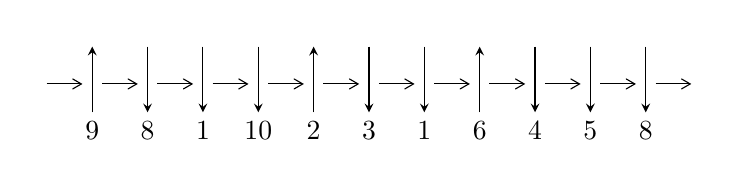
\begin{tikzpicture}[x=20pt, y=17pt]
	% nodes
	\node (C0) at (0, 0) {};
	\node (C1) at (1, 0) {};
	\node (C1U) at (1, +1) {};
	\node (C1D) at (1, -1) {9};

	\node (C2) at (2, 0) {};
	\node (C2U) at (2, +1) {};
	\node (C2D) at (2, -1) {8};

	\node (C3) at (3, 0) {};
	\node (C3U) at (3, +1) {};
	\node (C3D) at (3, -1) {1};

	\node (C4) at (4, 0) {};
	\node (C4U) at (4, +1) {};
	\node (C4D) at (4, -1) {10};

	\node (C5) at (5, 0) {};
	\node (C5U) at (5, +1) {};
	\node (C5D) at (5, -1) {2};

	\node (C6) at (6, 0) {};
	\node (C6U) at (6, +1) {};
	\node (C6D) at (6, -1) {3};

	\node (C7) at (7, 0) {};
	\node (C7U) at (7, +1) {};
	\node (C7D) at (7, -1) {1};

	\node (C8) at (8, 0) {};
	\node (C8U) at (8, +1) {};
	\node (C8D) at (8, -1) {6};

	\node (C9) at (9, 0) {};
	\node (C9U) at (9, +1) {};
	\node (C9D) at (9, -1) {4};

	\node (C10) at (10, 0) {};
	\node (C10U) at (10, +1) {};
	\node (C10D) at (10, -1) {5};

	\node (C11) at (11, 0) {};
	\node (C11U) at (11, +1) {};
	\node (C11D) at (11, -1) {8};
	\node (C12) at (12, 0) {};

	% arrows
	\draw[->,>={angle 60}]
	(C0) edge (C1) (C1) edge (C2) (C2) edge (C3) (C3) edge (C4) (C4) edge (C5) (C5) edge (C6) (C6) edge (C7) (C7) edge (C8) (C8) edge (C9) (C9) edge (C10) (C10) edge (C11) (C11) edge (C12) ;	\draw[->,>=stealth]
	(C1D) edge (C1U) (C2U) edge (C2D) (C3U) edge (C3D) (C4U) edge (C4D) (C5D) edge (C5U) (C6U) edge (C6D) (C7U) edge (C7D) (C8D) edge (C8U) (C9U) edge (C9D) (C10U) edge (C10D) (C11U) edge (C11D) ;
	\end{tikzpicture} \\
\hhline{~~} \\& 
\textbf{Solving Sequence} \\ \cline{2-2} 
 &
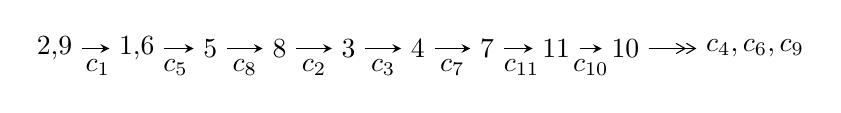
\begin{tikzpicture}[x=25pt, y=7pt]
	% node
	\node (A0) at (-1/8, 0) {2,9};
	\node (A1) at (17/16, 0) {1,6};
	\node (A2) at (17/8, 0) {5};
	\node (A3) at (25/8, 0) {8};
	\node (A4) at (33/8, 0) {3};
	\node (A5) at (41/8, 0) {4};
	\node (A6) at (49/8, 0) {7};
	\node (A7) at (57/8, 0) {11};
	\node (A8) at (65/8, 0) {10};
	\node (C1) at (1/2, -1) {$c_{1}$};
	\node (C2) at (13/8, -1) {$c_{5}$};
	\node (C3) at (21/8, -1) {$c_{8}$};
	\node (C4) at (29/8, -1) {$c_{2}$};
	\node (C5) at (37/8, -1) {$c_{3}$};
	\node (C6) at (45/8, -1) {$c_{7}$};
	\node (C7) at (53/8, -1) {$c_{11}$};
	\node (C8) at (61/8, -1) {$c_{10}$};
	\node (A9) at (10, 0) {$c_{4},c_{6},c_{9}$};

	% edge
	\draw[->,>=stealth]	
	(A0) edge (A1) (A1) edge (A2) (A2) edge (A3) (A3) edge (A4) (A4) edge (A5) (A5) edge (A6) (A6) edge (A7) (A7) edge (A8) ;
	\draw[->>,>={angle 60}]	
	(A8) edge (A9);
\end{tikzpicture} \\ 

\end{tabular} \\

\footnotetext{
The image of knot diagram is generated by the software ``\textbf{Draw programme}" developed by Andrew Bartholomew(\url{http://www.layer8.co.uk/maths/draw/index.htm\#Running-draw}), where we modified some parts for our purpose(\url{https://github.com/CATsTAILs/LinksPainter}).
}\phantom \\ \newline 
\centering \textbf{Ideals for irreducible components\footnotemark of $X_{\text{par}}$} 
 
\begin{align*}
I^u_{1}&=\langle 
b- u,\;-159345685747 u^{18}+147982590951 u^{17}+\cdots+96727442787 a+357093230263,\\
\phantom{I^u_{1}}&\phantom{= \langle  }u^{19}- u^{18}+\cdots- u+1\rangle \\
I^u_{2}&=\langle 
b+u,\;4343 u^{12}+7110 u^{11}+\cdots+4787 a+1912,\\
\phantom{I^u_{2}}&\phantom{= \langle  }u^{13}+u^{12}- u^{11}-3 u^{10}-2 u^9+u^8-2 u^6+u^5-4 u^4-2 u^3-2 u^2-1\rangle \\
I^u_{3}&=\langle 
1.31062\times10^{16} u^{15}-1.74217\times10^{16} u^{14}+\cdots+9.51505\times10^{17} b+6.50537\times10^{17},\\
\phantom{I^u_{3}}&\phantom{= \langle  }1.97533\times10^{15} u^{15}-3.11116\times10^{14} u^{14}+\cdots+5.49461\times10^{17} a+2.28716\times10^{17},\;u^{16}-3 u^{15}+\cdots+14 u+41\rangle \\
\\
\end{align*}
\raggedright * 3 irreducible components of $\dim_{\mathbb{C}}=0$, with total 48 representations.\\
\footnotetext{All coefficients of polynomials are rational numbers. But the coefficients are sometimes approximated in decimal forms when there is not enough margin.}
\newpage
\renewcommand{\arraystretch}{1}
\centering \section*{I. $I^u_{1}= \langle b- u,\;-1.59\times10^{11} u^{18}+1.48\times10^{11} u^{17}+\cdots+9.67\times10^{10} a+3.57\times10^{11},\;u^{19}- u^{18}+\cdots- u+1 \rangle$}
\flushleft \textbf{(i) Arc colorings}\\
\begin{tabular}{m{7pt} m{180pt} m{7pt} m{180pt} }
\flushright $a_{2}=$&$\begin{pmatrix}1\\0\end{pmatrix}$ \\
\flushright $a_{9}=$&$\begin{pmatrix}0\\u\end{pmatrix}$ \\
\flushright $a_{1}=$&$\begin{pmatrix}1\\u^2\end{pmatrix}$ \\
\flushright $a_{6}=$&$\begin{pmatrix}1.64737 u^{18}-1.52989 u^{17}+\cdots+32.1590 u-3.69175\\u\end{pmatrix}$ \\
\flushright $a_{5}=$&$\begin{pmatrix}1.64737 u^{18}-1.52989 u^{17}+\cdots+31.1590 u-3.69175\\u\end{pmatrix}$ \\
\flushright $a_{8}=$&$\begin{pmatrix}2.27741 u^{18}-2.43525 u^{17}+\cdots+37.2324 u-9.52801\\0.111340 u^{18}-0.0665068 u^{17}+\cdots+2.52989 u+0.117475\end{pmatrix}$ \\
\flushright $a_{3}=$&$\begin{pmatrix}-0.820898 u^{18}+0.672626 u^{17}+\cdots-23.6867 u-3.53398\\0.162954 u^{18}-0.347555 u^{17}+\cdots+0.470733 u-0.393621\end{pmatrix}$ \\
\flushright $a_{4}=$&$\begin{pmatrix}-1.01209 u^{18}+0.851055 u^{17}+\cdots-23.4848 u-2.99209\\0.340664 u^{18}-0.462435 u^{17}+\cdots+0.649162 u-0.380858\end{pmatrix}$ \\
\flushright $a_{7}=$&$\begin{pmatrix}2.55969 u^{18}-2.59941 u^{17}+\cdots+42.1976 u-9.56837\\-0.0125024 u^{18}-0.0176043 u^{17}+\cdots+2.36573 u-0.000645074\end{pmatrix}$ \\
\flushright $a_{11}=$&$\begin{pmatrix}2.20417 u^{18}-1.64059 u^{17}+\cdots+52.9687 u+7.25501\\-0.191192 u^{18}+0.178429 u^{17}+\cdots+0.201893 u+0.541893\end{pmatrix}$ \\
\flushright $a_{10}=$&$\begin{pmatrix}0.426507 u^{18}-0.339257 u^{17}+\cdots+12.4593 u+5.79766\\-0.340664 u^{18}+0.462435 u^{17}+\cdots-0.649162 u+0.380858\end{pmatrix}$\\ \flushright $a_{10}=$&$\begin{pmatrix}0.426507 u^{18}-0.339257 u^{17}+\cdots+12.4593 u+5.79766\\-0.340664 u^{18}+0.462435 u^{17}+\cdots-0.649162 u+0.380858\end{pmatrix}$\\&\end{tabular}
\flushleft \textbf{(ii) Obstruction class $= -1$}\\~\\
\flushleft \textbf{(iii) Cusp Shapes $= \frac{162836171512}{96727442787} u^{18}-\frac{43813217810}{32242480929} u^{17}+\cdots+\frac{1086609567736}{32242480929} u+\frac{428864721314}{96727442787}$}\\~\\
\newpage\renewcommand{\arraystretch}{1}
\flushleft \textbf{(iv) u-Polynomials at the component}\newline \\
\begin{tabular}{m{50pt}|m{274pt}}
Crossings & \hspace{64pt}u-Polynomials at each crossing \\
\hline $$\begin{aligned}c_{1},c_{5}\end{aligned}$$&$\begin{aligned}
&u^{19}- u^{18}+\cdots- u+1
\end{aligned}$\\
\hline $$\begin{aligned}c_{2}\end{aligned}$$&$\begin{aligned}
&u^{19}-10 u^{17}+\cdots+21 u+6
\end{aligned}$\\
\hline $$\begin{aligned}c_{3}\end{aligned}$$&$\begin{aligned}
&u^{19}-9 u^{18}+\cdots+52 u-16
\end{aligned}$\\
\hline $$\begin{aligned}c_{4},c_{9},c_{10}\end{aligned}$$&$\begin{aligned}
&u^{19}-9 u^{18}+\cdots-4 u^2+16
\end{aligned}$\\
\hline $$\begin{aligned}c_{6},c_{7},c_{11}\end{aligned}$$&$\begin{aligned}
&u^{19}+u^{18}+\cdots+2 u+1
\end{aligned}$\\
\hline $$\begin{aligned}c_{8}\end{aligned}$$&$\begin{aligned}
&u^{19}+9 u^{18}+\cdots+34 u+4
\end{aligned}$\\
\hline
\end{tabular}\\~\\
\newpage\renewcommand{\arraystretch}{1}
\flushleft \textbf{(v) Riley Polynomials at the component}\newline \\
\begin{tabular}{m{50pt}|m{274pt}}
Crossings & \hspace{64pt}Riley Polynomials at each crossing \\
\hline $$\begin{aligned}c_{1},c_{5}\end{aligned}$$&$\begin{aligned}
&y^{19}+15 y^{18}+\cdots-47 y-1
\end{aligned}$\\
\hline $$\begin{aligned}c_{2}\end{aligned}$$&$\begin{aligned}
&y^{19}-20 y^{18}+\cdots+273 y-36
\end{aligned}$\\
\hline $$\begin{aligned}c_{3}\end{aligned}$$&$\begin{aligned}
&y^{19}-25 y^{18}+\cdots+6064 y-256
\end{aligned}$\\
\hline $$\begin{aligned}c_{4},c_{9},c_{10}\end{aligned}$$&$\begin{aligned}
&y^{19}-17 y^{18}+\cdots+128 y-256
\end{aligned}$\\
\hline $$\begin{aligned}c_{6},c_{7},c_{11}\end{aligned}$$&$\begin{aligned}
&y^{19}-33 y^{18}+\cdots+12 y-1
\end{aligned}$\\
\hline $$\begin{aligned}c_{8}\end{aligned}$$&$\begin{aligned}
&y^{19}- y^{18}+\cdots-116 y-16
\end{aligned}$\\
\hline
\end{tabular}\\~\\
\newpage\flushleft \textbf{(vi) Complex Volumes and Cusp Shapes}
$$\begin{array}{c|c|c}  
\text{Solutions to }I^u_{1}& \I (\text{vol} + \sqrt{-1}CS) & \text{Cusp shape}\\
 \hline 
\begin{aligned}
u &= -0.074551 + 1.005150 I \\
a &= \phantom{-}0.755499 - 0.268182 I \\
b &= -0.074551 + 1.005150 I\end{aligned}
 & -6.47985 - 3.00781 I & -9.19206 + 3.40012 I \\ \hline\begin{aligned}
u &= -0.074551 - 1.005150 I \\
a &= \phantom{-}0.755499 + 0.268182 I \\
b &= -0.074551 - 1.005150 I\end{aligned}
 & -6.47985 + 3.00781 I & -9.19206 - 3.40012 I \\ \hline\begin{aligned}
u &= \phantom{-}0.719291 + 0.870215 I \\
a &= \phantom{-}0.618624 + 0.041528 I \\
b &= \phantom{-}0.719291 + 0.870215 I\end{aligned}
 & -0.22723 + 2.57483 I & -7.79227 - 4.00370 I \\ \hline\begin{aligned}
u &= \phantom{-}0.719291 - 0.870215 I \\
a &= \phantom{-}0.618624 - 0.041528 I \\
b &= \phantom{-}0.719291 - 0.870215 I\end{aligned}
 & -0.22723 - 2.57483 I & -7.79227 + 4.00370 I \\ \hline\begin{aligned}
u &= -0.015666 + 1.186340 I \\
a &= \phantom{-}1.00740 - 1.04818 I \\
b &= -0.015666 + 1.186340 I\end{aligned}
 & -8.13053 + 0.97689 I & -10.22917 - 0.27205 I \\ \hline\begin{aligned}
u &= -0.015666 - 1.186340 I \\
a &= \phantom{-}1.00740 + 1.04818 I \\
b &= -0.015666 - 1.186340 I\end{aligned}
 & -8.13053 - 0.97689 I & -10.22917 + 0.27205 I \\ \hline\begin{aligned}
u &= -0.799079\phantom{ +0.000000I} \\
a &= -0.714422\phantom{ +0.000000I} \\
b &= -0.799079\phantom{ +0.000000I}\end{aligned}
 & -1.52055\phantom{ +0.000000I} & -7.33430\phantom{ +0.000000I} \\ \hline\begin{aligned}
u &= -0.197897 + 0.643434 I \\
a &= -0.839512 + 0.061465 I \\
b &= -0.197897 + 0.643434 I\end{aligned}
 & -0.928589 + 0.684123 I & -8.21629 - 4.45735 I \\ \hline\begin{aligned}
u &= -0.197897 - 0.643434 I \\
a &= -0.839512 - 0.061465 I \\
b &= -0.197897 - 0.643434 I\end{aligned}
 & -0.928589 - 0.684123 I & -8.21629 + 4.45735 I \\ \hline\begin{aligned}
u &= -0.78204 + 1.18371 I \\
a &= -0.553988 + 0.003237 I \\
b &= -0.78204 + 1.18371 I\end{aligned}
 & -5.79784 - 5.72974 I & -14.4693 + 5.0563 I\\
 \hline 
 \end{array}$$\newpage$$\begin{array}{c|c|c}  
\text{Solutions to }I^u_{1}& \I (\text{vol} + \sqrt{-1}CS) & \text{Cusp shape}\\
 \hline 
\begin{aligned}
u &= -0.78204 - 1.18371 I \\
a &= -0.553988 - 0.003237 I \\
b &= -0.78204 - 1.18371 I\end{aligned}
 & -5.79784 + 5.72974 I & -14.4693 - 5.0563 I \\ \hline\begin{aligned}
u &= -0.58654 + 1.32638 I \\
a &= -1.071040 - 0.314706 I \\
b &= -0.58654 + 1.32638 I\end{aligned}
 & -8.63276 - 7.82560 I & -8.78089 + 5.39108 I \\ \hline\begin{aligned}
u &= -0.58654 - 1.32638 I \\
a &= -1.071040 + 0.314706 I \\
b &= -0.58654 - 1.32638 I\end{aligned}
 & -8.63276 + 7.82560 I & -8.78089 - 5.39108 I \\ \hline\begin{aligned}
u &= \phantom{-}0.70619 + 1.27768 I \\
a &= -0.185916 - 1.077090 I \\
b &= \phantom{-}0.70619 + 1.27768 I\end{aligned}
 & -15.6607 + 4.6824 I & -10.38940 - 2.40952 I \\ \hline\begin{aligned}
u &= \phantom{-}0.70619 - 1.27768 I \\
a &= -0.185916 + 1.077090 I \\
b &= \phantom{-}0.70619 - 1.27768 I\end{aligned}
 & -15.6607 - 4.6824 I & -10.38940 + 2.40952 I \\ \hline\begin{aligned}
u &= \phantom{-}0.050654 + 0.205531 I \\
a &= -4.15202 + 6.06789 I \\
b &= \phantom{-}0.050654 + 0.205531 I\end{aligned}
 & \phantom{-}2.26122 + 2.63337 I & \phantom{-}2.15678 + 7.21953 I \\ \hline\begin{aligned}
u &= \phantom{-}0.050654 - 0.205531 I \\
a &= -4.15202 - 6.06789 I \\
b &= \phantom{-}0.050654 - 0.205531 I\end{aligned}
 & \phantom{-}2.26122 - 2.63337 I & \phantom{-}2.15678 - 7.21953 I \\ \hline\begin{aligned}
u &= \phantom{-}1.08010 + 1.60653 I \\
a &= \phantom{-}0.778162 - 0.084178 I \\
b &= \phantom{-}1.08010 + 1.60653 I\end{aligned}
 & -16.5060 + 12.7254 I & -9.92028 - 5.57941 I \\ \hline\begin{aligned}
u &= \phantom{-}1.08010 - 1.60653 I \\
a &= \phantom{-}0.778162 + 0.084178 I \\
b &= \phantom{-}1.08010 - 1.60653 I\end{aligned}
 & -16.5060 - 12.7254 I & -9.92028 + 5.57941 I\\
 \hline 
 \end{array}$$\newpage\newpage\renewcommand{\arraystretch}{1}
\centering \section*{II. $I^u_{2}= \langle b+u,\;4343 u^{12}+7110 u^{11}+\cdots+4787 a+1912,\;u^{13}+u^{12}+\cdots-2 u^2-1 \rangle$}
\flushleft \textbf{(i) Arc colorings}\\
\begin{tabular}{m{7pt} m{180pt} m{7pt} m{180pt} }
\flushright $a_{2}=$&$\begin{pmatrix}1\\0\end{pmatrix}$ \\
\flushright $a_{9}=$&$\begin{pmatrix}0\\u\end{pmatrix}$ \\
\flushright $a_{1}=$&$\begin{pmatrix}1\\u^2\end{pmatrix}$ \\
\flushright $a_{6}=$&$\begin{pmatrix}-0.907249 u^{12}-1.48527 u^{11}+\cdots+1.45874 u-0.399415\\- u\end{pmatrix}$ \\
\flushright $a_{5}=$&$\begin{pmatrix}-0.907249 u^{12}-1.48527 u^{11}+\cdots+2.45874 u-0.399415\\- u\end{pmatrix}$ \\
\flushright $a_{8}=$&$\begin{pmatrix}-1.64216 u^{12}-2.04115 u^{11}+\cdots+2.52663 u-1.91936\\0.199081 u^{12}+0.339043 u^{11}+\cdots+0.0927512 u-0.578024\end{pmatrix}$ \\
\flushright $a_{3}=$&$\begin{pmatrix}-0.578024 u^{12}-1.37894 u^{11}+\cdots+1.60058 u+2.09275\\-0.300606 u^{12}-0.253812 u^{11}+\cdots-0.757050 u+0.0963025\end{pmatrix}$ \\
\flushright $a_{4}=$&$\begin{pmatrix}-0.137456 u^{12}-0.933988 u^{11}+\cdots+1.77961 u+1.19553\\-0.604972 u^{12}-0.393357 u^{11}+\cdots-0.316482 u+0.100689\end{pmatrix}$ \\
\flushright $a_{7}=$&$\begin{pmatrix}-1.74493 u^{12}-2.58450 u^{11}+\cdots+4.26154 u-2.09839\\0.194694 u^{12}+0.639022 u^{11}+\cdots-0.0100272 u-1.01859\end{pmatrix}$ \\
\flushright $a_{11}=$&$\begin{pmatrix}-0.399415 u^{12}-1.30666 u^{11}+\cdots+5.21370 u+2.45874\\0.440568 u^{12}+0.444955 u^{11}+\cdots+0.179027 u-0.897222\end{pmatrix}$ \\
\flushright $a_{10}=$&$\begin{pmatrix}0.374556 u^{12}+0.339879 u^{11}+\cdots+1.20389 u+1.04470\\0.604972 u^{12}+0.393357 u^{11}+\cdots+0.316482 u-0.100689\end{pmatrix}$\\ \flushright $a_{10}=$&$\begin{pmatrix}0.374556 u^{12}+0.339879 u^{11}+\cdots+1.20389 u+1.04470\\0.604972 u^{12}+0.393357 u^{11}+\cdots+0.316482 u-0.100689\end{pmatrix}$\\&\end{tabular}
\flushleft \textbf{(ii) Obstruction class $= 1$}\\~\\
\flushleft \textbf{(iii) Cusp Shapes $= \frac{14164}{4787} u^{12}+\frac{37634}{4787} u^{11}+\cdots-\frac{78472}{4787} u-\frac{64919}{4787}$}\\~\\
\newpage\renewcommand{\arraystretch}{1}
\flushleft \textbf{(iv) u-Polynomials at the component}\newline \\
\begin{tabular}{m{50pt}|m{274pt}}
Crossings & \hspace{64pt}u-Polynomials at each crossing \\
\hline $$\begin{aligned}c_{1},c_{5}\end{aligned}$$&$\begin{aligned}
&u^{13}+u^{12}- u^{11}-3 u^{10}-2 u^9+u^8-2 u^6+u^5-4 u^4-2 u^3-2 u^2-1
\end{aligned}$\\
\hline $$\begin{aligned}c_{2}\end{aligned}$$&$\begin{aligned}
&u^{13}-3 u^{11}-2 u^{10}+3 u^9+u^8-9 u^7-11 u^6+u^5-2 u^4-10 u^3-3 u^2-1
\end{aligned}$\\
\hline $$\begin{aligned}c_{3}\end{aligned}$$&$\begin{aligned}
&u^{13}+10 u^{12}+\cdots+19 u+5
\end{aligned}$\\
\hline $$\begin{aligned}c_{4}\end{aligned}$$&$\begin{aligned}
&u^{13}-7 u^{11}+\cdots+2 u+1
\end{aligned}$\\
\hline $$\begin{aligned}c_{6},c_{11}\end{aligned}$$&$\begin{aligned}
&u^{13}- u^{12}+\cdots+u-1
\end{aligned}$\\
\hline $$\begin{aligned}c_{7}\end{aligned}$$&$\begin{aligned}
&u^{13}+u^{12}+\cdots+u+1
\end{aligned}$\\
\hline $$\begin{aligned}c_{8}\end{aligned}$$&$\begin{aligned}
&u^{13}-6 u^{12}+\cdots-5 u^2+1
\end{aligned}$\\
\hline $$\begin{aligned}c_{9},c_{10}\end{aligned}$$&$\begin{aligned}
&u^{13}-7 u^{11}+\cdots+2 u-1
\end{aligned}$\\
\hline
\end{tabular}\\~\\
\newpage\renewcommand{\arraystretch}{1}
\flushleft \textbf{(v) Riley Polynomials at the component}\newline \\
\begin{tabular}{m{50pt}|m{274pt}}
Crossings & \hspace{64pt}Riley Polynomials at each crossing \\
\hline $$\begin{aligned}c_{1},c_{5}\end{aligned}$$&$\begin{aligned}
&y^{13}-3 y^{12}+\cdots-4 y-1
\end{aligned}$\\
\hline $$\begin{aligned}c_{2}\end{aligned}$$&$\begin{aligned}
&y^{13}-6 y^{12}+\cdots-6 y-1
\end{aligned}$\\
\hline $$\begin{aligned}c_{3}\end{aligned}$$&$\begin{aligned}
&y^{13}-18 y^{12}+\cdots-59 y-25
\end{aligned}$\\
\hline $$\begin{aligned}c_{4},c_{9},c_{10}\end{aligned}$$&$\begin{aligned}
&y^{13}-14 y^{12}+\cdots+12 y-1
\end{aligned}$\\
\hline $$\begin{aligned}c_{6},c_{7},c_{11}\end{aligned}$$&$\begin{aligned}
&y^{13}-7 y^{12}+\cdots-9 y-1
\end{aligned}$\\
\hline $$\begin{aligned}c_{8}\end{aligned}$$&$\begin{aligned}
&y^{13}-2 y^{12}+\cdots+10 y-1
\end{aligned}$\\
\hline
\end{tabular}\\~\\
\newpage\flushleft \textbf{(vi) Complex Volumes and Cusp Shapes}
$$\begin{array}{c|c|c}  
\text{Solutions to }I^u_{2}& \I (\text{vol} + \sqrt{-1}CS) & \text{Cusp shape}\\
 \hline 
\begin{aligned}
u &= \phantom{-}0.900740 + 0.533669 I \\
a &= -1.166450 - 0.261249 I \\
b &= -0.900740 - 0.533669 I\end{aligned}
 & \phantom{-}1.59640 + 3.38566 I & \phantom{-}2.41525 - 6.49353 I \\ \hline\begin{aligned}
u &= \phantom{-}0.900740 - 0.533669 I \\
a &= -1.166450 + 0.261249 I \\
b &= -0.900740 + 0.533669 I\end{aligned}
 & \phantom{-}1.59640 - 3.38566 I & \phantom{-}2.41525 + 6.49353 I \\ \hline\begin{aligned}
u &= \phantom{-}0.134578 + 0.883277 I \\
a &= -1.058690 - 0.319537 I \\
b &= -0.134578 - 0.883277 I\end{aligned}
 & -8.02879 - 2.87155 I & -15.3113 + 3.5915 I \\ \hline\begin{aligned}
u &= \phantom{-}0.134578 - 0.883277 I \\
a &= -1.058690 + 0.319537 I \\
b &= -0.134578 + 0.883277 I\end{aligned}
 & -8.02879 + 2.87155 I & -15.3113 - 3.5915 I \\ \hline\begin{aligned}
u &= -0.529571 + 0.532870 I \\
a &= \phantom{-}0.059596 - 1.149930 I \\
b &= \phantom{-}0.529571 - 0.532870 I\end{aligned}
 & -5.39720 + 0.76633 I & -5.46823 + 1.57837 I \\ \hline\begin{aligned}
u &= -0.529571 - 0.532870 I \\
a &= \phantom{-}0.059596 + 1.149930 I \\
b &= \phantom{-}0.529571 + 0.532870 I\end{aligned}
 & -5.39720 - 0.76633 I & -5.46823 - 1.57837 I \\ \hline\begin{aligned}
u &= -1.310290 + 0.394846 I \\
a &= \phantom{-}0.714514 - 0.488710 I \\
b &= \phantom{-}1.310290 - 0.394846 I\end{aligned}
 & -1.52980 - 2.82140 I & -9.56946 + 2.96660 I \\ \hline\begin{aligned}
u &= -1.310290 - 0.394846 I \\
a &= \phantom{-}0.714514 + 0.488710 I \\
b &= \phantom{-}1.310290 + 0.394846 I\end{aligned}
 & -1.52980 + 2.82140 I & -9.56946 - 2.96660 I \\ \hline\begin{aligned}
u &= -0.736626 + 1.155190 I \\
a &= \phantom{-}0.633923 + 0.241978 I \\
b &= \phantom{-}0.736626 - 1.155190 I\end{aligned}
 & -4.89940 - 5.64504 I & -5.13604 + 4.51836 I \\ \hline\begin{aligned}
u &= -0.736626 - 1.155190 I \\
a &= \phantom{-}0.633923 - 0.241978 I \\
b &= \phantom{-}0.736626 + 1.155190 I\end{aligned}
 & -4.89940 + 5.64504 I & -5.13604 - 4.51836 I\\
 \hline 
 \end{array}$$\newpage$$\begin{array}{c|c|c}  
\text{Solutions to }I^u_{2}& \I (\text{vol} + \sqrt{-1}CS) & \text{Cusp shape}\\
 \hline 
\begin{aligned}
u &= \phantom{-}0.266732 + 0.548396 I \\
a &= -1.77971 + 1.81477 I \\
b &= -0.266732 - 0.548396 I\end{aligned}
 & \phantom{-}2.09623 + 2.92285 I & -9.7624 - 12.7438 I \\ \hline\begin{aligned}
u &= \phantom{-}0.266732 - 0.548396 I \\
a &= -1.77971 - 1.81477 I \\
b &= -0.266732 + 0.548396 I\end{aligned}
 & \phantom{-}2.09623 - 2.92285 I & -9.7624 + 12.7438 I \\ \hline\begin{aligned}
u &= \phantom{-}1.54888\phantom{ +0.000000I} \\
a &= \phantom{-}0.193632\phantom{ +0.000000I} \\
b &= -1.54888\phantom{ +0.000000I}\end{aligned}
 & -13.7330\phantom{ +0.000000I} & -11.3360\phantom{ +0.000000I}\\
 \hline 
 \end{array}$$\newpage\newpage\renewcommand{\arraystretch}{1}
\centering \section*{III. $I^u_{3}= \langle 1.31\times10^{16} u^{15}-1.74\times10^{16} u^{14}+\cdots+9.52\times10^{17} b+6.51\times10^{17},\;1.98\times10^{15} u^{15}-3.11\times10^{14} u^{14}+\cdots+5.49\times10^{17} a+2.29\times10^{17},\;u^{16}-3 u^{15}+\cdots+14 u+41 \rangle$}
\flushleft \textbf{(i) Arc colorings}\\
\begin{tabular}{m{7pt} m{180pt} m{7pt} m{180pt} }
\flushright $a_{2}=$&$\begin{pmatrix}1\\0\end{pmatrix}$ \\
\flushright $a_{9}=$&$\begin{pmatrix}0\\u\end{pmatrix}$ \\
\flushright $a_{1}=$&$\begin{pmatrix}1\\u^2\end{pmatrix}$ \\
\flushright $a_{6}=$&$\begin{pmatrix}-0.00359503 u^{15}+0.000566220 u^{14}+\cdots-0.579421 u-0.416256\\-0.0137742 u^{15}+0.0183096 u^{14}+\cdots-1.40476 u-0.683692\end{pmatrix}$ \\
\flushright $a_{5}=$&$\begin{pmatrix}0.0101791 u^{15}-0.0177434 u^{14}+\cdots+0.825342 u+0.267436\\-0.0137742 u^{15}+0.0183096 u^{14}+\cdots-1.40476 u-0.683692\end{pmatrix}$ \\
\flushright $a_{8}=$&$\begin{pmatrix}0.00188225 u^{15}+0.00703654 u^{14}+\cdots-0.906661 u+0.946317\\0.00958945 u^{15}-0.0187823 u^{14}+\cdots+0.0486549 u+0.591789\end{pmatrix}$ \\
\flushright $a_{3}=$&$\begin{pmatrix}-0.0135877 u^{15}+0.0698365 u^{14}+\cdots-0.200013 u+1.71159\\0.00578290 u^{15}-0.00717672 u^{14}+\cdots+1.12471 u+0.593614\end{pmatrix}$ \\
\flushright $a_{4}=$&$\begin{pmatrix}-0.0142111 u^{15}+0.0554273 u^{14}+\cdots-1.17466 u-0.0740275\\0.0136940 u^{15}-0.0307409 u^{14}+\cdots+1.37818 u+1.26107\end{pmatrix}$ \\
\flushright $a_{7}=$&$\begin{pmatrix}0.0120905 u^{15}-0.00811315 u^{14}+\cdots-0.603268 u+2.05812\\0.000452209 u^{15}-0.00935974 u^{14}+\cdots-0.586534 u-0.0426882\end{pmatrix}$ \\
\flushright $a_{11}=$&$\begin{pmatrix}0.0142111 u^{15}-0.0554273 u^{14}+\cdots+1.17466 u+0.0740275\\-0.000623414 u^{15}-0.0144091 u^{14}+\cdots-0.974645 u-1.78562\end{pmatrix}$ \\
\flushright $a_{10}=$&$\begin{pmatrix}0.0101791 u^{15}-0.0177434 u^{14}+\cdots+0.825342 u+0.267436\\-0.000703594 u^{15}-0.0268404 u^{14}+\cdots-0.00122333 u-1.20825\end{pmatrix}$\\ \flushright $a_{10}=$&$\begin{pmatrix}0.0101791 u^{15}-0.0177434 u^{14}+\cdots+0.825342 u+0.267436\\-0.000703594 u^{15}-0.0268404 u^{14}+\cdots-0.00122333 u-1.20825\end{pmatrix}$\\&\end{tabular}
\flushleft \textbf{(ii) Obstruction class $= -1$}\\~\\
\flushleft \textbf{(iii) Cusp Shapes $= \frac{1227691828059108}{13401481882079569} u^{15}-\frac{4398465163137376}{13401481882079569} u^{14}+\cdots+\frac{68931370501080476}{13401481882079569} u-\frac{199658948531840914}{13401481882079569}$}\\~\\
\newpage\renewcommand{\arraystretch}{1}
\flushleft \textbf{(iv) u-Polynomials at the component}\newline \\
\begin{tabular}{m{50pt}|m{274pt}}
Crossings & \hspace{64pt}u-Polynomials at each crossing \\
\hline $$\begin{aligned}c_{1},c_{5}\end{aligned}$$&$\begin{aligned}
&u^{16}-3 u^{15}+\cdots+14 u+41
\end{aligned}$\\
\hline $$\begin{aligned}c_{2}\end{aligned}$$&$\begin{aligned}
&u^{16}- u^{15}+\cdots-398 u+359
\end{aligned}$\\
\hline $$\begin{aligned}c_{3}\end{aligned}$$&$\begin{aligned}
&(u^4+3 u^3+u^2-2 u+1)^4
\end{aligned}$\\
\hline $$\begin{aligned}c_{4},c_{9},c_{10}\end{aligned}$$&$\begin{aligned}
&(u^2+u-1)^8
\end{aligned}$\\
\hline $$\begin{aligned}c_{6},c_{7},c_{11}\end{aligned}$$&$\begin{aligned}
&u^{16}- u^{15}+\cdots-314 u+59
\end{aligned}$\\
\hline $$\begin{aligned}c_{8}\end{aligned}$$&$\begin{aligned}
&(u^4- u^3+u^2+1)^4
\end{aligned}$\\
\hline
\end{tabular}\\~\\
\newpage\renewcommand{\arraystretch}{1}
\flushleft \textbf{(v) Riley Polynomials at the component}\newline \\
\begin{tabular}{m{50pt}|m{274pt}}
Crossings & \hspace{64pt}Riley Polynomials at each crossing \\
\hline $$\begin{aligned}c_{1},c_{5}\end{aligned}$$&$\begin{aligned}
&y^{16}- y^{15}+\cdots+6528 y+1681
\end{aligned}$\\
\hline $$\begin{aligned}c_{2}\end{aligned}$$&$\begin{aligned}
&y^{16}-13 y^{15}+\cdots-519558 y+128881
\end{aligned}$\\
\hline $$\begin{aligned}c_{3}\end{aligned}$$&$\begin{aligned}
&(y^4-7 y^3+15 y^2-2 y+1)^4
\end{aligned}$\\
\hline $$\begin{aligned}c_{4},c_{9},c_{10}\end{aligned}$$&$\begin{aligned}
&(y^2-3 y+1)^8
\end{aligned}$\\
\hline $$\begin{aligned}c_{6},c_{7},c_{11}\end{aligned}$$&$\begin{aligned}
&y^{16}-21 y^{15}+\cdots-63668 y+3481
\end{aligned}$\\
\hline $$\begin{aligned}c_{8}\end{aligned}$$&$\begin{aligned}
&(y^4+y^3+3 y^2+2 y+1)^4
\end{aligned}$\\
\hline
\end{tabular}\\~\\
\newpage\flushleft \textbf{(vi) Complex Volumes and Cusp Shapes}
$$\begin{array}{c|c|c}  
\text{Solutions to }I^u_{3}& \I (\text{vol} + \sqrt{-1}CS) & \text{Cusp shape}\\
 \hline 
\begin{aligned}
u &= \phantom{-}0.070726 + 1.109990 I \\
a &= -0.866375 + 0.712201 I \\
b &= -0.71670 - 1.63688 I\end{aligned}
 & -7.02670 + 3.16396 I & -10.17326 - 2.56480 I \\ \hline\begin{aligned}
u &= \phantom{-}0.070726 - 1.109990 I \\
a &= -0.866375 - 0.712201 I \\
b &= -0.71670 + 1.63688 I\end{aligned}
 & -7.02670 - 3.16396 I & -10.17326 + 2.56480 I \\ \hline\begin{aligned}
u &= \phantom{-}0.779961 + 0.810134 I \\
a &= \phantom{-}0.678421 + 0.218895 I \\
b &= \phantom{-}2.29306 - 1.45821 I\end{aligned}
 & -14.02850 + 1.41510 I & -13.8267 - 4.9087 I \\ \hline\begin{aligned}
u &= \phantom{-}0.779961 - 0.810134 I \\
a &= \phantom{-}0.678421 - 0.218895 I \\
b &= \phantom{-}2.29306 + 1.45821 I\end{aligned}
 & -14.02850 - 1.41510 I & -13.8267 + 4.9087 I \\ \hline\begin{aligned}
u &= -0.749741 + 0.435456 I \\
a &= \phantom{-}1.37743 - 0.41545 I \\
b &= \phantom{-}0.996480 - 0.636712 I\end{aligned}
 & \phantom{-}0.86898 - 3.16396 I & -10.17326 + 2.56480 I \\ \hline\begin{aligned}
u &= -0.749741 - 0.435456 I \\
a &= \phantom{-}1.37743 + 0.41545 I \\
b &= \phantom{-}0.996480 + 0.636712 I\end{aligned}
 & \phantom{-}0.86898 + 3.16396 I & -10.17326 - 2.56480 I \\ \hline\begin{aligned}
u &= \phantom{-}0.996480 + 0.636712 I \\
a &= -1.021930 - 0.261538 I \\
b &= -0.749741 - 0.435456 I\end{aligned}
 & \phantom{-}0.86898 + 3.16396 I & -10.17326 - 2.56480 I \\ \hline\begin{aligned}
u &= \phantom{-}0.996480 - 0.636712 I \\
a &= -1.021930 + 0.261538 I \\
b &= -0.749741 + 0.435456 I\end{aligned}
 & \phantom{-}0.86898 - 3.16396 I & -10.17326 + 2.56480 I \\ \hline\begin{aligned}
u &= -0.062069 + 0.700905 I \\
a &= -1.063840 - 0.407726 I \\
b &= -1.11172 - 0.94845 I\end{aligned}
 & -6.13277 - 1.41510 I & -13.8267 + 4.9087 I \\ \hline\begin{aligned}
u &= -0.062069 - 0.700905 I \\
a &= -1.063840 + 0.407726 I \\
b &= -1.11172 + 0.94845 I\end{aligned}
 & -6.13277 + 1.41510 I & -13.8267 - 4.9087 I\\
 \hline 
 \end{array}$$\newpage$$\begin{array}{c|c|c}  
\text{Solutions to }I^u_{3}& \I (\text{vol} + \sqrt{-1}CS) & \text{Cusp shape}\\
 \hline 
\begin{aligned}
u &= -1.11172 + 0.94845 I \\
a &= \phantom{-}0.136782 - 0.531259 I \\
b &= -0.062069 - 0.700905 I\end{aligned}
 & -6.13277 + 1.41510 I & -13.8267 - 4.9087 I \\ \hline\begin{aligned}
u &= -1.11172 - 0.94845 I \\
a &= \phantom{-}0.136782 + 0.531259 I \\
b &= -0.062069 + 0.700905 I\end{aligned}
 & -6.13277 - 1.41510 I & -13.8267 + 4.9087 I \\ \hline\begin{aligned}
u &= -0.71670 + 1.63688 I \\
a &= \phantom{-}0.658359 + 0.232127 I \\
b &= \phantom{-}0.070726 - 1.109990 I\end{aligned}
 & -7.02670 - 3.16396 I & -10.17326 + 2.56480 I \\ \hline\begin{aligned}
u &= -0.71670 - 1.63688 I \\
a &= \phantom{-}0.658359 - 0.232127 I \\
b &= \phantom{-}0.070726 + 1.109990 I\end{aligned}
 & -7.02670 + 3.16396 I & -10.17326 - 2.56480 I \\ \hline\begin{aligned}
u &= \phantom{-}2.29306 + 1.45821 I \\
a &= -0.033000 - 0.293154 I \\
b &= \phantom{-}0.779961 - 0.810134 I\end{aligned}
 & -14.02850 - 1.41510 I & -13.8267 + 4.9087 I \\ \hline\begin{aligned}
u &= \phantom{-}2.29306 - 1.45821 I \\
a &= -0.033000 + 0.293154 I \\
b &= \phantom{-}0.779961 + 0.810134 I\end{aligned}
 & -14.02850 + 1.41510 I & -13.8267 - 4.9087 I\\
 \hline 
 \end{array}$$\newpage
\newpage\renewcommand{\arraystretch}{1}
\centering \section*{ IV. u-Polynomials}
\begin{tabular}{m{50pt}|m{274pt}}
Crossings & \hspace{64pt}u-Polynomials at each crossing \\
\hline $$\begin{aligned}c_{1},c_{5}\end{aligned}$$&$\begin{aligned}
&(u^{13}+u^{12}- u^{11}-3 u^{10}-2 u^9+u^8-2 u^6+u^5-4 u^4-2 u^3-2 u^2-1)\\
&\cdot(u^{16}-3 u^{15}+\cdots+14 u+41)(u^{19}- u^{18}+\cdots- u+1)
\end{aligned}$\\
\hline $$\begin{aligned}c_{2}\end{aligned}$$&$\begin{aligned}
&(u^{13}-3 u^{11}-2 u^{10}+3 u^9+u^8-9 u^7-11 u^6+u^5-2 u^4-10 u^3-3 u^2-1)\\
&\cdot(u^{16}- u^{15}+\cdots-398 u+359)(u^{19}-10 u^{17}+\cdots+21 u+6)
\end{aligned}$\\
\hline $$\begin{aligned}c_{3}\end{aligned}$$&$\begin{aligned}
&((u^4+3 u^3+u^2-2 u+1)^4)(u^{13}+10 u^{12}+\cdots+19 u+5)\\
&\cdot(u^{19}-9 u^{18}+\cdots+52 u-16)
\end{aligned}$\\
\hline $$\begin{aligned}c_{4}\end{aligned}$$&$\begin{aligned}
&((u^2+u-1)^8)(u^{13}-7 u^{11}+\cdots+2 u+1)(u^{19}-9 u^{18}+\cdots-4 u^2+16)
\end{aligned}$\\
\hline $$\begin{aligned}c_{6},c_{11}\end{aligned}$$&$\begin{aligned}
&(u^{13}- u^{12}+\cdots+u-1)(u^{16}- u^{15}+\cdots-314 u+59)\\
&\cdot(u^{19}+u^{18}+\cdots+2 u+1)
\end{aligned}$\\
\hline $$\begin{aligned}c_{7}\end{aligned}$$&$\begin{aligned}
&(u^{13}+u^{12}+\cdots+u+1)(u^{16}- u^{15}+\cdots-314 u+59)\\
&\cdot(u^{19}+u^{18}+\cdots+2 u+1)
\end{aligned}$\\
\hline $$\begin{aligned}c_{8}\end{aligned}$$&$\begin{aligned}
&((u^4- u^3+u^2+1)^4)(u^{13}-6 u^{12}+\cdots-5 u^2+1)\\
&\cdot(u^{19}+9 u^{18}+\cdots+34 u+4)
\end{aligned}$\\
\hline $$\begin{aligned}c_{9},c_{10}\end{aligned}$$&$\begin{aligned}
&((u^2+u-1)^8)(u^{13}-7 u^{11}+\cdots+2 u-1)(u^{19}-9 u^{18}+\cdots-4 u^2+16)
\end{aligned}$\\
\hline
\end{tabular}\newpage\renewcommand{\arraystretch}{1}
\centering \section*{ V. Riley Polynomials}
\begin{tabular}{m{50pt}|m{274pt}}
Crossings & \hspace{64pt}Riley Polynomials at each crossing \\
\hline $$\begin{aligned}c_{1},c_{5}\end{aligned}$$&$\begin{aligned}
&(y^{13}-3 y^{12}+\cdots-4 y-1)(y^{16}- y^{15}+\cdots+6528 y+1681)\\
&\cdot(y^{19}+15 y^{18}+\cdots-47 y-1)
\end{aligned}$\\
\hline $$\begin{aligned}c_{2}\end{aligned}$$&$\begin{aligned}
&(y^{13}-6 y^{12}+\cdots-6 y-1)(y^{16}-13 y^{15}+\cdots-519558 y+128881)\\
&\cdot(y^{19}-20 y^{18}+\cdots+273 y-36)
\end{aligned}$\\
\hline $$\begin{aligned}c_{3}\end{aligned}$$&$\begin{aligned}
&((y^4-7 y^3+15 y^2-2 y+1)^4)(y^{13}-18 y^{12}+\cdots-59 y-25)\\
&\cdot(y^{19}-25 y^{18}+\cdots+6064 y-256)
\end{aligned}$\\
\hline $$\begin{aligned}c_{4},c_{9},c_{10}\end{aligned}$$&$\begin{aligned}
&((y^2-3 y+1)^8)(y^{13}-14 y^{12}+\cdots+12 y-1)\\
&\cdot(y^{19}-17 y^{18}+\cdots+128 y-256)
\end{aligned}$\\
\hline $$\begin{aligned}c_{6},c_{7},c_{11}\end{aligned}$$&$\begin{aligned}
&(y^{13}-7 y^{12}+\cdots-9 y-1)(y^{16}-21 y^{15}+\cdots-63668 y+3481)\\
&\cdot(y^{19}-33 y^{18}+\cdots+12 y-1)
\end{aligned}$\\
\hline $$\begin{aligned}c_{8}\end{aligned}$$&$\begin{aligned}
&((y^4+y^3+3 y^2+2 y+1)^4)(y^{13}-2 y^{12}+\cdots+10 y-1)\\
&\cdot(y^{19}- y^{18}+\cdots-116 y-16)
\end{aligned}$\\
\hline
\end{tabular}
\vskip 2pc
\end{document}